%!TEX root = mieic-en.tex

\chapter{Literature Review} \label{chap:sota}

\section*{}
\textit{
Neste capítulo é descrito o estado da arte e são
apresentados trabalhos relacionados para mostrar o que existe no
mesmo domínio e quais os problemas em aberto.
Deve deixar claro que existe uma oportunidade de desenvolvimento que
cobre alguma falha concreta .
O capítulo deve também efetuar uma revisão tecnológica às principais
ferramentas utilizáveis no âmbito do projeto, justificando futuras
escolhas.
}

Resenha utilizaçao computer vision em trafego e em transportes
Concluir com os desafios da armis (drive, quere aplicaro computer vision para automatizar determinados aspetos)
Sequência de funcionalidades que respondem ao desafio da Armis(segmentaçao,deteçao,...)
Uma secção para cada um

Tese Gustavo Lira / Pedro Loureiro

\section{History of Computer Vision}

Computer vision appeared as an area of investigation around the mid 60's at the MIT by Professor Larry Roberts, whose PhD. thesis focused on methods to extract 3D information from a 2D image ~\cite{huang_computer_1996} in order to reconstruct entire scenes from the geometry gathered. This area is now considered by the ACM as a branch of artificial intelligence according to the 2012 ACM Computing Classification System ~\cite{acm_2012_2012}. From this point onward scientists began applying the techniques developed in multiple fields.

The use of computer vision in manufacturing industry was among the first to be explored, as there were already multiple robots working in the assembly lines of the factories that needed to be improved, as noted by Stout in 1980 ~\cite{stout_computer_1980}. These robots were becoming outdated due to the lack of interaction with the environment. This meant that for a robot to work with a part in an assembly line it needed to be placed in a pre-determined position, and any deviation could mean that the line needed to be stopped. Michael Baird relates in ~\cite{l._baird_sight-i:_1978} a computer vision system developed to inspect circuit chips rotation deviation in a welding base, indicating to the welder that the chip needed to be adjusted. Computer vision was also used as a tool to automatically analyse weather satellite images ~\cite{binford_computer_1973-2} and multidimensional medical images ~\cite{ayache_medical_1998}, with applications being developed in these areas being now common in our daily life.

\subsection{Computer Vision in Intelligent Transport Systems}

Regarding intelligent transport systems (ITSs), the use of computer vision to aid in the analysis of traffic has been increasing in the last years due to the decreasing costs of hardware, both cameras, storage and processing power, as well as the growing knowledge to extract useful data from the video gathered. In contrast to the high installation and upkeep costs of other traffic control tools such as Inductive Loop Detectors and Microwave Vehicle Detectors, applying computer vision to handle these tasks is a profitable option for entities in charge of the analysis of this data.

One of the first works applying computer vision to analyse traffic was published in 1984 ~\cite{dickinson_image_1984} and detected and measured movement in a sequence of frames. Since then, multiple fields of study have been created, not only for the measuring of traffic, as explored in ~\cite{lira_computer-vision_2016}, ~\cite{buch_review_2011-1} and ~\cite{hashmi_analysis_2012} where the authors evaluate methods to analyse traffic in urban environments, but also for the analysis of the environment around a self-driven vehicle, reading traffic signs using multiple approaches using convolutional neural networks ~\cite{soendoro_traffic_2011} or using bag-of-visual-words ~\cite{supriyanto_unsupervised_2016}, or to automatize the parking process as discussed in ~\cite{hammoudi_self-driven_2016}. Recently some studies have surfaced where the authors discuss the analysis of passenger numbers and behaviour inside vehicles, in order to enforce traffic laws ~\cite{loce_detection_2017-1}.

For our application however we need to focus on the aspect of traffic analysis, and in order to understand what traffic analysis software needs to accomplish, it is convenient to study what composes a typical traffic scene. Usually the scenes are viewed from a top-down perspective that places the cars against the road as background, as seen in ~\ref{fig:hh_traffic}. The vehicles have a roughly regular rectangular shape when viewed from the top, with little variation when the camera is rotated, however their textures vary heavily, making it difficult for a detector to work based on the vehicles image representation ~\cite{badenas_applying_1998}. However, depending on the camera position there can be object occlusion by other objects or scene components, which makes it difficult to detect and track vehicles relying solely on subtraction based segmentation techniques.

\begin{figure}[h]
  \begin{center}
    \leavevmode
    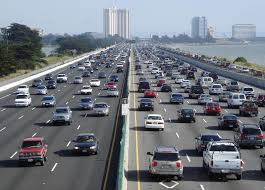
\includegraphics[width=0.5\textwidth]{traffic_scene}
    \caption{Typical High-Way Traffic Scene}
    \label{fig:hh_traffic}
  \end{center}
\end{figure}

The scenes also have varying light according to the time of the day, and proposed solutions need to adapt to these changes as fast as possible, otherwise data might be lost. Other weather conditions can also interfere with the analysis, such as fog and rain, and need to be addressed when designing solutions.

\subsection{Our Challenge}

The "Analytics Server" module of the "Video Server" project had a list of requirements that needed to be \todo{Acabar}

Detetar eventos relevantes
	Contra mao
	Objetos caidos

Contar Veiculos

Apenas para camaras fixas


\section{Foreground Segmentation}

Image segmentation is the process through which  an image is separated into its different regions according to the desired output, usually objects of interest. These regions are composed by pixels that have a common characteristic ~\cite{shapiro_computer_2001} dependant on the desired result. There are several ways one can accomplish an adequate segmentation of an image, and the most relevant ones to our purpose are described below.

\subsection{Background Subtraction}

Background Subtraction is a segmentation technique based on the analysis of the difference of consecutive frames and use that information to create a background model, a representation of what the image looks like without any moving objects present. Given the nature of the process, cameras must be static and although some research has been made to overcome this issue ~\cite{li_detection_2012} ~\cite{sheikh_background_2009} ~\cite{zamalieva_background_2014}, this is beyond the scope of the project, due to the requirements given.

There are however a number of different ways to implement the background subtraction developed across the years with increasing segmentation accuracy and computational performance. Piccardi presented an overview of the most relevant ones in ~\cite{piccardi_background_2004}, aiming to present each method's strengths and weaknesses. From this work we can present a list of the algorithms considered for implementation in the project.

\subsubsection{Frame Differencing}

This is the simplest approach to the problem as it only considers two frames at a time, making it only work in certain scenarios where the speed of the objects and frame rate of the camera allow it. In this model a pixel is considered as foreground if it satisfies the equation presented in ~\ref{eq:frame_diff}, and since the only parametrizable value is the Threshold, the whole segmentation process is very sensitive to any changes in this value.

\begin{eqnarray}
\label{eq:frame_diff}
\left | frame_{i} - frame_{i-1} \right | >= Threshold
\end{eqnarray}
\subsubsection{History Based Background Model}

In order to make this segmentation method more robust, in the early 2000's Velastin ~\cite{lo_automatic_2001} and Cucchiara ~\cite{cucchiara_detecting_2003} proposed a mathematical model to take into consideration past frames when calculating the Background Model of the scene. The most simple version of the improved algorithm used a running average of the past frames as seen in ~\ref{eq:running_average}. This eliminates the need to store the frames in memory as the new average can be calculated using the previous results.

\begin{eqnarray}
\label{eq:running_average}
BackgroundModel _{i+1} = \alpha * Frame_{i} + (1-\alpha)* BackgroundModel _{i}
\end{eqnarray}

Instead of the running average one can use the median value of the last n frames, improving the method reaction to outlying values. In both however, the history can be just the n frames or a weighted average where recent frames have more weight. Both these methods cannot cope with intermittent changes on the background, such as moving leaves against a building facade, and to solve this problem a new approach was proposed, the Mixture of Gaussians which models each pixel according to a mixture of Gaussian distributions, usually 3 to 5, but in later research ~\cite{zivkovic_improved_2004} a method was developed to calculate the number of distributions needed on a per pixel basis.

\subsection{Object Based}

Object Based segmentation relies on the a priori knowledge of the geometry of the objects we want to extract from the image. It is mainly used in medical applications such as in ~\cite{snell_model-based_1993} where it is used to extract a model of the brain surface from MRI scans \todo{Acabar}

\section{Image Treatment}

This section will review some of the proposed methods to improve image quality before or during processing by removing noise, extracting unwanted features or enhancing relevant features for the processes involved.

\subsection{Blur}

In order to blur an image one needs to convolve it using a special kind of filter. The process of convolution in image processing consists in the application of a filter to every pixel of an image, returning a new image where each pixel is the result of the function to the pixel in the same position in the previous image. As we can see in ~\ref{fig:convolution} the application of a 3*3 mask, where all 9 values have the value 1/9, results in a image where each pixel value equals the mean of itself and surrounding neighbours in the original image.

\begin{figure}[h]
  \begin{center}
    \leavevmode
    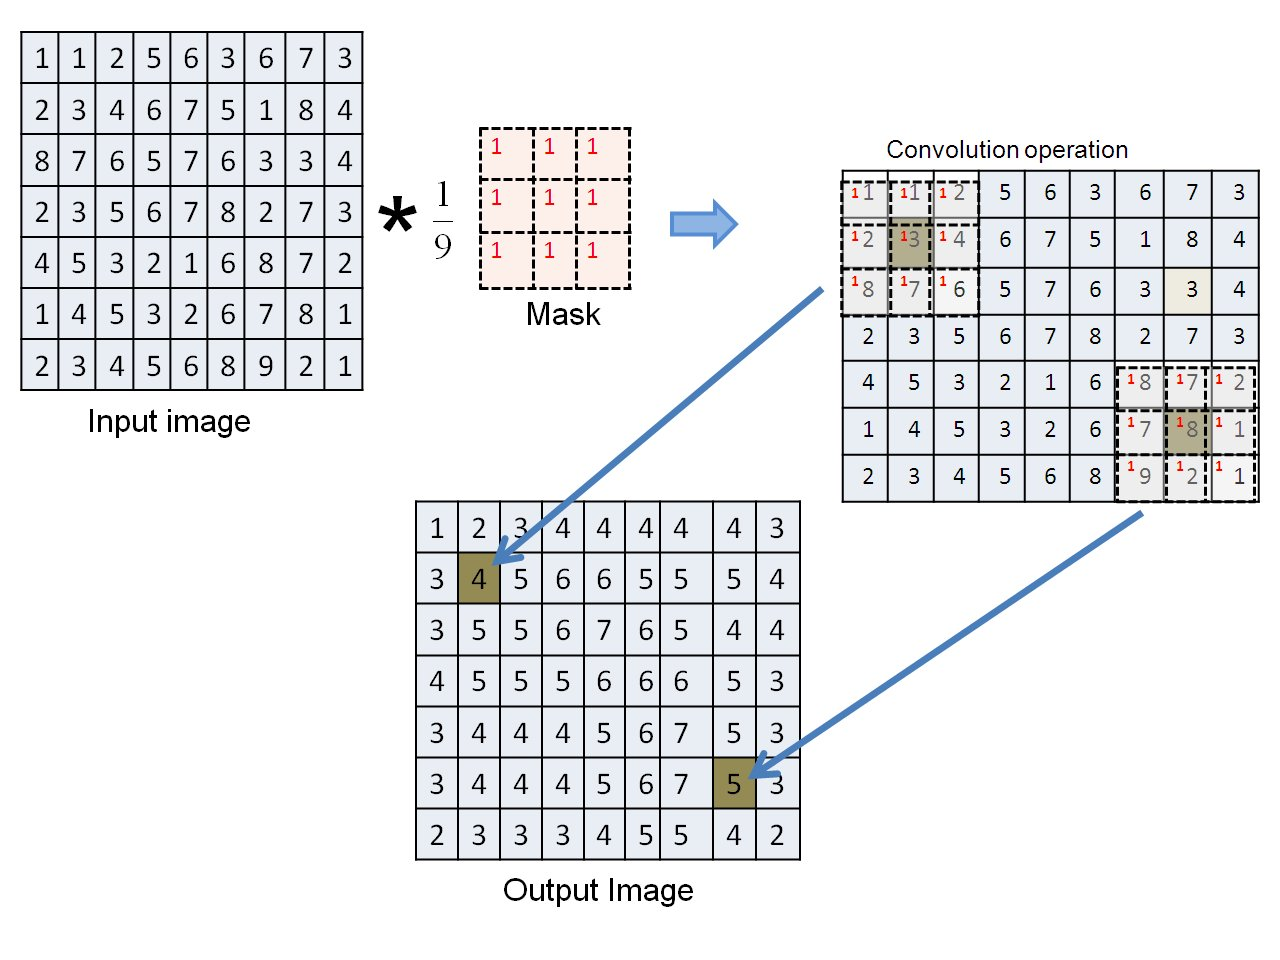
\includegraphics[width=0.7\textwidth]{convolution}
    \caption{Convolution Example ~\cite{labs_theory_2017}}
    \label{fig:convolution}
  \end{center}
\end{figure}

While this is the simplest blur processing we can apply to an image, there are more complex ones that yield better results. The one most often used in image processing is the Gaussian Blur, which uses a square filter with values calculated with the equation in ~\ref{eq:gaussian} from ~\cite{shapiro_computer_2001}.

\begin{eqnarray}
\label{eq:gaussian}
G(x,y) = \frac{1}{2\pi \sigma ^{2}}e^{-\frac{x^{2}+y^{2}}{2\sigma ^{2}}}
\end{eqnarray}

This equation returns a filter consisting of concentric circles that results in a smooth blurring of the images due to the application of the same power of blurring from equidistant pixels. The function can be tuned to the needs of the process through the $\sigma$ value, returning a sharper or softer blur filter as seen in figure ~\ref{fig:gaussian}.

\begin{figure}[h]
  \begin{center}
    \leavevmode
    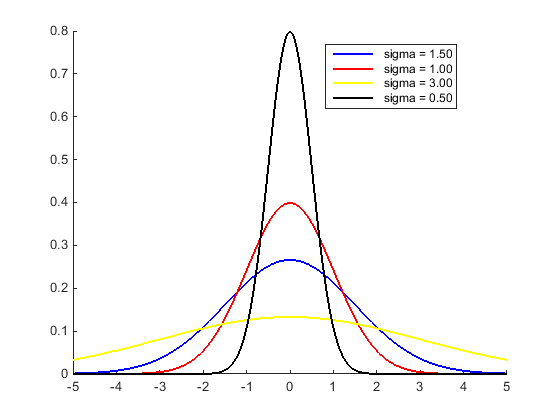
\includegraphics[width=0.5\textwidth]{gaussian}
    \caption{Gaussian Function Variation with Sigma Value}
    \label{fig:gaussian}
  \end{center}
\end{figure}

This kind of filters have multiple uses in computer vision. Blurring an image removes the grain noise it contains, creating more even surfaces that ease the process of image processing, as well as making edges easier to detect with edge detection algorithms.

\subsection{Edge Detection}

Detecting the edges in an image is an important step into the understanding of its contents, allowing segmentation based on surfaces and a spatial perception of the scene. The work presented by Marr and Hildreth ~\cite{Marr1980TheoryOE} defines edges as part visual and part physical and proceeds to show that the two are interconnected. The first step of the proposed process is to calculate the zero-crossings of equation ~\ref{eq:intensity}, the Laplacian of a two dimensional Gaussian applied to different scales of the image, which returns both the points of intensity change and the slopes of the function at that point.

\begin{eqnarray}
\label{eq:intensity}
\nabla^{2} G(x,y)*I(x,y)
\end{eqnarray}

What the authors noted was that if an edge was detected at a certain scale it appears also at adjacent scales, which they called "spatial coincidence assumption". This theory can be reversed, if there is a convergence of edges on multiple scales there is a real physical edge, and based on this, if we find zero-crossings on neighbour scales, we can assume there is a real edge in that region. From here multiple implementations of the algorithm appeared, the most used one being presented below, the Canny Edge Detector using a Sobel filter. Although this was among the first implementations of an edge detector it is still the state-of-the-art process and is used regularly in a variety of applications

The Sobel filter is used to create an image that accentuates the edges of an original image. This process works by convolving two kernels with the image, one for the horizontal and the other for the vertical direction, that return the intesity change in that pixel for each one. The filters can be seen in ~\ref{eq:sobel_filter} as they were presented by Irwin Sobel ~\cite{sobel_isotropic_1989}.

\begin{eqnarray}
\label{eq:sobel_filter}
G_{x} =
\begin{bmatrix}
+1 & 0 & -1\\ 
+2 & 0 & -2\\ 
+1 & 0 & -1
\end{bmatrix}  G_{y} = \begin{bmatrix}
+1 & +2 & +1\\ 
0 & 0 & 0\\ 
-1 & -2 & -1
\end{bmatrix}
\end{eqnarray}

Using $G_{x}$ and $G_{y}$ it is possible to retrieve the regions of the image that contain edges by calculating the magnitude of the gradient vector as the square root of the sum of the squares of both components and thresholding these values. One of the features of this process is the ability to retrieve the direction of the edge from these values, using the inverse tangent operation.

The Canny Edge Detector uses the result of the Sobel filter as input and filters the most relevant edges as well as thinning them to 1-pixel wide lines. To accomplish this Canny used an optimization process comparing the value of the gradient magnitude to the one of the neighbour pixels along the direction returned by the Sobel filter, and keeping only the one with the largest value along the edge.

\subsection{Morphology Operators}


\subsection{Shadow Removal}
Rain Removal
Shadow Removal

\section{Secção Exemplo}\label{sec:dialecto}

\emph{Scalable Vector Graphics}\index{SVG}\index{XML!SVG} é uma
linguagem em formato XML que descreve gráficos de duas dimensões. 
Este formato padronizado pela W3C (\emph{World Wide Web Consortium})
é livre de patentes ou direitos de autor e está totalmente
documentado, à semelhança de outros W3C
standards~cite{kn:svgdoc}.

Sendo uma linguagem XML, o \svg{} herda uma série de vantagens: a
possibilidade de transformar \svg{} usando técnicas como
XSLT\index{XML!XSLT}, de embeber \svg{} em qualquer documento
XML\index{XML} usando \textit{namespaces} ou até de  
estilizar \svg{} recorrendo a CSS\index{CSS} (\emph{Cascade Style Sheets}). 
De uma forma geral, pode dizer-se que \svg{}s interagem bem com as
atuais tecnologias ligadas ao XML e à Web, tal como referido
em~cite{kn:svgibm,kn:svgw3c}.

\section{Resumo ou Conclusões}

No final do capítulo deverá ser apresentado um resumo com as 
principais conclusões que se podem tirar. 

Vivamus non nunc nec risus tempor varius. Quisque bibendum mi at
dolor. Aliquam consectetuer condimentum risus. Aliquam luctus pulvinar
sem. Duis aliquam, urna et vulputate tristique, dui elit aliquet nibh,
vel dignissim magna turpis id sapien. Duis commodo sem id
quam. Phasellus dolor. Class aptent taciti sociosqu ad litora torquent
per conubia nostra, per inceptos himenaeos. 
